%----------------------------------------------------%
%                    INTRODUCCION                    %
%----------------------------------------------------%

\pagestyle{fancy}

\chapter{Introducción}
\label{introduccion}

Desde Aristóteles y su libro Segundos Analíticos \footnote{\href{https://docs.google.com/a/datik.es/file/d/0By4kcbi6MzzdUHhVQnUtcTNUdk0/view}{Órganon II de Aristóteles: Recopilación de obras Aristotélicas que incluye el libro Segundo Analíticos}} hasta Galileo, padre de la ciencia moderna, adalides del conocimiento han proclamado que un método de investigación basado en lo empírico y en la medición, sujeto a los principios específicos de las pruebas de razonamiento es el camino para conocer la verdad.\\

Hoy en día, época en la que los avances tecnológicos han posibilitado observar y medir de forma exhaustiva un gran abanico de fenómenos, la ingente cantidad de datos que se genera en el proceso es, a veces, intratable mediante las tecnologías convencionales, y por ende, es imposible extraer todo el conocimiento que atesoran. El problema, lejos de atenuarse, se acrecienta con el paso del tiempo. Estudios como el realizado por McKinsey Global Institute \footnote{\href{http://www.mckinsey.com/mgi/overview}{McKinsey Global Institute}} estiman que el volumen de datos que se genera crece un 40\% cada año y auguran que entre 2009 y 2020 se verá multiplicado por 44 \cite{nambiartowards}.\\

Para lidiar con dicha problemática, en los últimos años ha irrumpido la necesidad de desarrollar nuevas metodologías y tecnologías que permitan operar eficientemente sobre masas colosales de datos, dando como resultado el nacimiento del Big Data \cite{manyika2011big}.\\

Empresas de renombre mundial, conscientes de los beneficios que el Big Data les puede reportar en diferentes facetas de su modelo de negocio, ya se han interesado en este fenómeno. De un estudio realizado entre los altos ejecutivos de las firmas que lideran el Wall Street se desprende que el 96\% tiene planeadas ciertas iniciativas relacionadas con el Big Data, y el 80\% ya tiene finalizada alguna \cite{bdes:2013}. 

\section{Contexto}
 
Datik Información Inteligente \footnote{\url{http://www.datik.es/}} es una empresa tecnológica perteneciente al Grupo Irizar \footnote{\url{http://www.irizar.com/irizar/}}  que desarrolla soluciones ITS destinadas a la gestión del trasporte, tanto ferroviario como por carretera y movilidad ciudadana.\\

Uno de los productos estrella de la entidad es el denominado iPanel, concentrador de  información que ofrece al operador de transporte servicios de valor añadido en la gestión de la información generada por su flota. El funcionamiento del servicio se puede resumir mediante la Figura \ref{fig:ipanel}:\\

\begin{figure}[h]
	\centering
	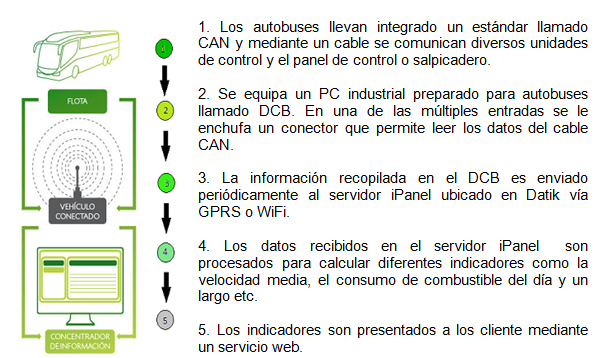
\includegraphics[width=1\textwidth]{Ilustraciones/ipanel_infraesctructure.png}
	\caption{Funcionamiento resumido de iPanel}
	\label{fig:ipanel}
\end{figure}

La incesante integración de nuevos vehículos en iPanel ha generado un crecimiento exponencial del número de registros almacenados en ciertas tablas MySQL. Aunque el volumen actual no llega a suponer riesgo alguno para el funcionamiento del servicio, Datik tiene identificados varios escenarios en los que la situación se podría revertir, causando graves inconvenientes.\\

Uno de los problemas, intrínseco a operar sobre una base de datos centralizada, es el denominado punto único de fallo o SPOF. Al tratarse del punto en el cual todos los procesos confluyen, el bloqueo o la caída causada por uno puede afectar al resto. Para mitigar los riesgos que ello conlleva, Datik ha optado por migrar su arquitectura monolítica a una basada en Microservicios \cite{newman2015building}, logrando así aislar los procesos que conforman sus servicios y mejorar ostensiblemente la estabilidad del sistema. No obstante, dicho cambio no soluciona los problemas inherentes a un proceso, que en caso de caída puede llegar a acarrear un funcionamiento inesperado de otros.\\ 

Fiel reflejo de ello es el Cálculo de Indicadores: proceso de ejecución diaria que realiza operaciones aritméticas intensivas sobre datos almacenados en diversas tablas para después, agrupar los resultados en base a diferentes criterios. Siendo dichas tablas las que mayor crecimiento experimentan, el aumento del volumen de las mismas incrementa de forma desorbitada el tiempo necesario para finalizar el cálculo, pudiendo, en un futuro, llegar a tardar más de 24 horas y cancelar los indicadores que ofrecen información del último día.\\

El objetivo del presente proyecto es proponer soluciones tecnológicas que solvente permanentemente el problema del proceso Cálculo de Indicadores y que a su vez, pueda valer para lidiar con otros obstáculos de la misma índole que pudieran emerger en un futuro.\\

\section{Propuesta}

Tal y como se ha mencionado en apartados anteriores, la problemática que envuelve al Cálculo de Indicadores es originado por el incremento exponencial de datos que dicho proceso ha de tratar. No sería descabellado pensar que la solución podría pasar por escalar verticalmente la máquina y afinar la configuración de MySQL. No obstante, ambas mejoras son limitadas, mientras que el volumen de los datos seguirá en aumento de forma inexorable, volviendo, tarde o temprano, a tener que lidiar con los mismos problemas del principio.\\

Siendo imposible reconducir la situación mediante las tecnologías tradicionales, en el presente proyecto se propone realizar un cambio de paradigma que implica migrar las tablas relacionadas con los Indicadores a un modelo distribuido que posibilite escalar la infraestructura horizontalmente. A su vez, se sugiere dividir el problema en dos apartados, almacenamiento y procesado, dotando la infraestructura de tecnología adecuada para ofrecer una respuesta eficaz a cada una de las partes.\\

En cuanto a almacenamiento se refiere, teniendo en cuenta que los datos a tratar no presentan relación alguna con el resto de las entidades, se propone utilizar una base de datos no relacional. Dentro de la extensa gama de sistemas de almacenamiento NoSQL \footnote{\url{http://nosql-database.org/}} existentes hoy en día, se ha considerado que Apache Cassandra \cite{lakshman2010cassandra} es el idóneo para solventar el problema gracias a que ofrece una disponibilidad total y un ratio de escrituras por segundo sustancialmente superior en comparación a sus homólogos \cite{rabl2012solving}.\\

Por su parte, para trabajar con el apartado del procesamiento se apuesta por Apache Spark \cite{zaharia2010spark}. Se trata de una plataforma de computación en clúster que ofrece una interfaz para programar operaciones paralelizadas y tolerantes a fallo que ha irrumpido con fuerza en el último lustro. A logrado desbancar tecnologías semejantes como MapReduce \cite{dean2008mapreduce} gracias a la capacidad de almacenar en memoria los resultados intermedios del cómputo posibilitando así acelerar el procesamiento hasta 100 veces \cite{xin2013shark} en determinados escenarios.\\

Para cuantificar los beneficios aportados por las tecnologías propuestas, teniendo en cuenta que Datik actualmente almacena una cantidad limitada de datos y que además estos se encuentran sujetos a una clausula de confidencialidad, se ha decidido hacer uso de un Dataset público de aproximadamente 25 GB que recoge la información de los trayectos realizados por los taxis amarillos de Nueva York durante el año 2015. \footnote{\url{http://www.nyc.gov/html/tlc/html/about/trip_record_data.shtml}}

\section{Organización del documento}

La presente memoria recoge el estudio empírico realizado sobre el rendimiento ofrecido por varias tecnologías emergentes en el campo del Big Data en comparación a una base de datos tradicional a la hora de operar en escenarios que requieren un almacenamiento y procesamiento eficaz de volúmenes masivos de datos.\\

En este primer capítulo se ha introducido la problemática que ha impulsado la creación del presente proyecto y se ha expuesto la propuesta para dar solución a la misma.\\

En el capítulo 2 se desgrana el funcionamiento de Apache Cassandra y Apache Spark, haciendo especial hincapié en aquellos aspectos que denotan una mejora sustancial en comparación a la arquitectura centralizada.\\

Una vez en el capítulo 3 se describen los entornos de prueba confeccionados para cuantificar la mejora 

explica la gestión llevada a cabo durante el proyecto. Se presentan las metodologías utilizadas: Metodologías Ágiles e InterMod (adaptada a las necesidades de este proyecto). A continuación se detallan cada una de las iteraciones llevadas a cabo (como parte de la metodología InterMod): duración, objetivos y tareas realizadas. Al final del capítulo se muestra la documentación asociada a las iteraciones y los objetivos, además del seguimiento de tiempo realizado.\\

A continuación, en el capítulo 4 se detalla el análisis de requisitos. Primero se detallan los requisitos no-funcionales y luego los funcionales (prototipos en papel llevados a cabo durante las primeras iteraciones que dan una visión global del proyecto).\\

En el capítulo 5 se explica el diseño e implementación llevados a cabo. Se comienza mostrando la estructura de documentos del proyecto, luego el diseño realizado en base al análisis de requisitos del capítulo 4 y finalmente una visión general de la implementación de la lógica de negocio.\\

Para finalizar, en el capítulo 6 se presentan las conclusiones, líneas futuras para el proyecto y las lecciones aprendidas.\\

Fuera de la estructura general de la memoria, tenemos la bibliografia y los apéndices. En estos últimos tenemos las actas de reuniones, las actas de pruebas y la vista de relaciones de la base de datos (de la parte utilizada o creada específicamente para el proyecto).\\